
\section{Implementation}
\label{sec:implementation}

We plan to implement the proposed approach in a programming
tool, whose general workflow is sketched in Figure~\ref{fig:workflow}.

\begin{figure}[t]
  \centering
  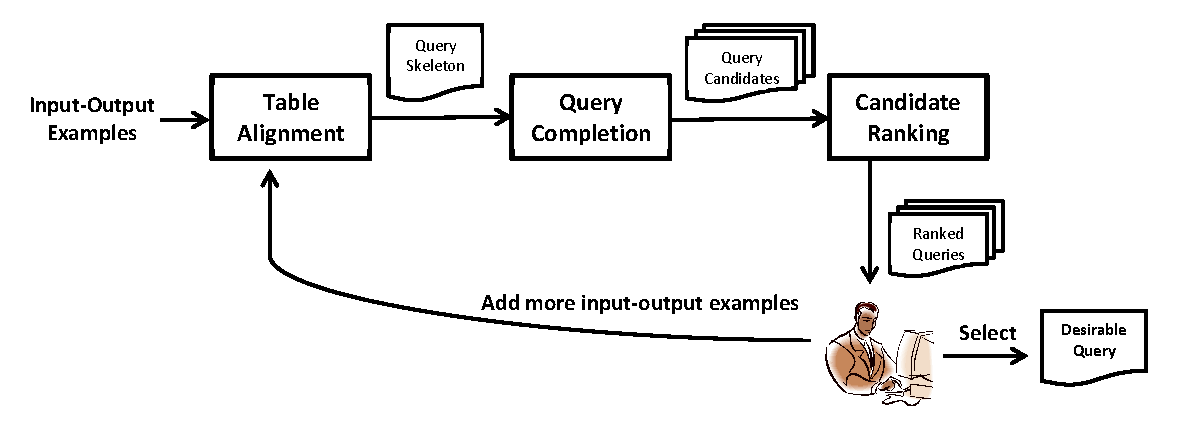
\includegraphics[scale=0.46]{workflow}
  \vspace*{-5.0ex}\caption {{\label{fig:workflow} The workflow of our SQL synthesis tool.
}}
\end{figure}

Our tool takes as input a pair of input-output example. It first performs
table alignment to infer a partially-complete query skeleton. The inferred query
skeleton, although contains unknown parts as holes, serves as good guidance
for inferring a complete SQL query.
Our tool then uses the search strategy defined in Section~\ref{sec:completion}
to fill this partial query, and possibly produces a list of query candidates.
Differing from a query skeleton, a query candidate is a valid, complete SQL query which satisfies
the provided input-output example. However, for a realistic problem,
multiple query candidates can satisfy the provided input-output example, and then be
generated. Our tool next ranks the candidate
query list, and provides users a ranked list of SQL queries with the most likely
ones on the top. This makes our tool more usable.

Our tool also takes the user interaction model (Section~\ref{sec:uim}) into account.
A user could either select a desirable query from the output ranked list if she is
satisified with the results, or provide
the tool additional examples to let the tool infer more accurate queries.

In our implementation, we choose MySQL as the backend database engine, which takes an
inferred SQL query candidate, executes it on the input tables, and checks whether the
output result matches the given output example.

